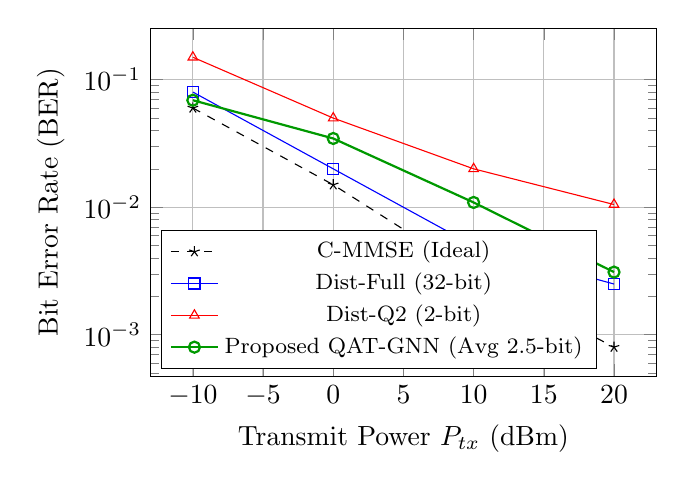
\begin{tikzpicture}
\begin{semilogyaxis}[
    xlabel={Transmit Power $P_{tx}$ (dBm)},
    ylabel={Bit Error Rate (BER)},
    grid=major,
    legend style={at={(0.02,0.02)}, anchor=south west, font=\footnotesize},
    cycle list name=color list,
    width=8cm,
    height=6cm
]

% C-MMSE (Upper Bound)
\addplot[color=black, mark=star, dashed] coordinates {
    (-10, 0.06) (0, 0.015) (10, 0.003) (20, 0.0008)
};
\addlegendentry{C-MMSE (Ideal)}

% Dist-Full (32-bit)
\addplot[color=blue, mark=square] coordinates {
    (-10, 0.08) (0, 0.02) (10, 0.005) (20, 0.0025)
};
\addlegendentry{Dist-Full (32-bit)}

% Dist-Q2 (2-bit)
\addplot[color=red, mark=triangle] coordinates {
    (-10, 0.15) (0, 0.05) (10, 0.02) (20, 0.0105)
};
\addlegendentry{Dist-Q2 (2-bit)}

% Proposed QAT-GNN (2.5-bit)
\addplot[color=green!60!black, mark=o, thick] coordinates {
    (-10, 0.069) (0, 0.0346) (10, 0.0109) (20, 0.0031)
};
\addlegendentry{Proposed QAT-GNN (Avg 2.5-bit)}

\end{semilogyaxis}
\end{tikzpicture}